%&latex
\documentclass{article}
\usepackage{commons/commons}
\usepackage{commons/note_style}

\usepackage{comment}
%\excludecomment{figure}

\def\ojoin{\setbox0=\hbox{$\bowtie$}%
  \rule[-.02ex]{.25em}{.4pt}\llap{\rule[\ht0]{.25em}{.4pt}}}
\def\leftouterjoin{\mathbin{\ojoin\mkern-5.8mu\bowtie}}
\def\rightouterjoin{\mathbin{\bowtie\mkern-5.8mu\ojoin}}
\def\fullouterjoin{\mathbin{\ojoin\mkern-5.8mu\bowtie\mkern-5.8mu\ojoin}}
\usepackage{amsbsy}
\usepackage{amstext}

\begin{document}

%+Title
\title{Advanced Database Quicksheet}
\author{Daniel D. Zhang}
\date{Fall 2015}
\maketitle
%-Title

%+Abstract
%\begin{abstract}
%This is the notes for CSE 232A.
%\end{abstract}
%-Abstract

%+Contents
\tableofcontents
%-Contents
\newpage

\section*{Preclude}
\begin{itemize}
\item \textbf{NULL}: NULL means absence of value. Any value \textbf{cannot} ever be $=$ (or $<>$) NULL because NULL has no value. However, SQL has special IS NULL and IS NOT NULL predicates for dealing with NULL.
\end{itemize}
\section*{Acronyms}
\
\begin{obeylines}
\rih{Attr}. Attributes 
\rih{Ptr}. Pointer
\rih{Mgt}. Management 
\end{obeylines}
\section{Introduction}
\begin{itemize}
\item Basic SQLs 
\item \rih{ACID}: Atomicity, Consistency, Isolation, Durability 
\begin{enumerate}
\item Atomicity: each transaction be "all or nothing".
\item Consistency: any transaction will bring the database from one valid state to
another.
\item Isolation: the concurrent execution of transactions results in a system state
that would be obtained if transactions were executed serially
\item Durability: once a transaction has been committed, it will remain so, even in
the event of power loss, crashes, or 
\end{enumerate}
\item Transaction Mgt
\item Database System Architecture. Fig:
\begin{figure}[hbtp]
\centering
\subfloat{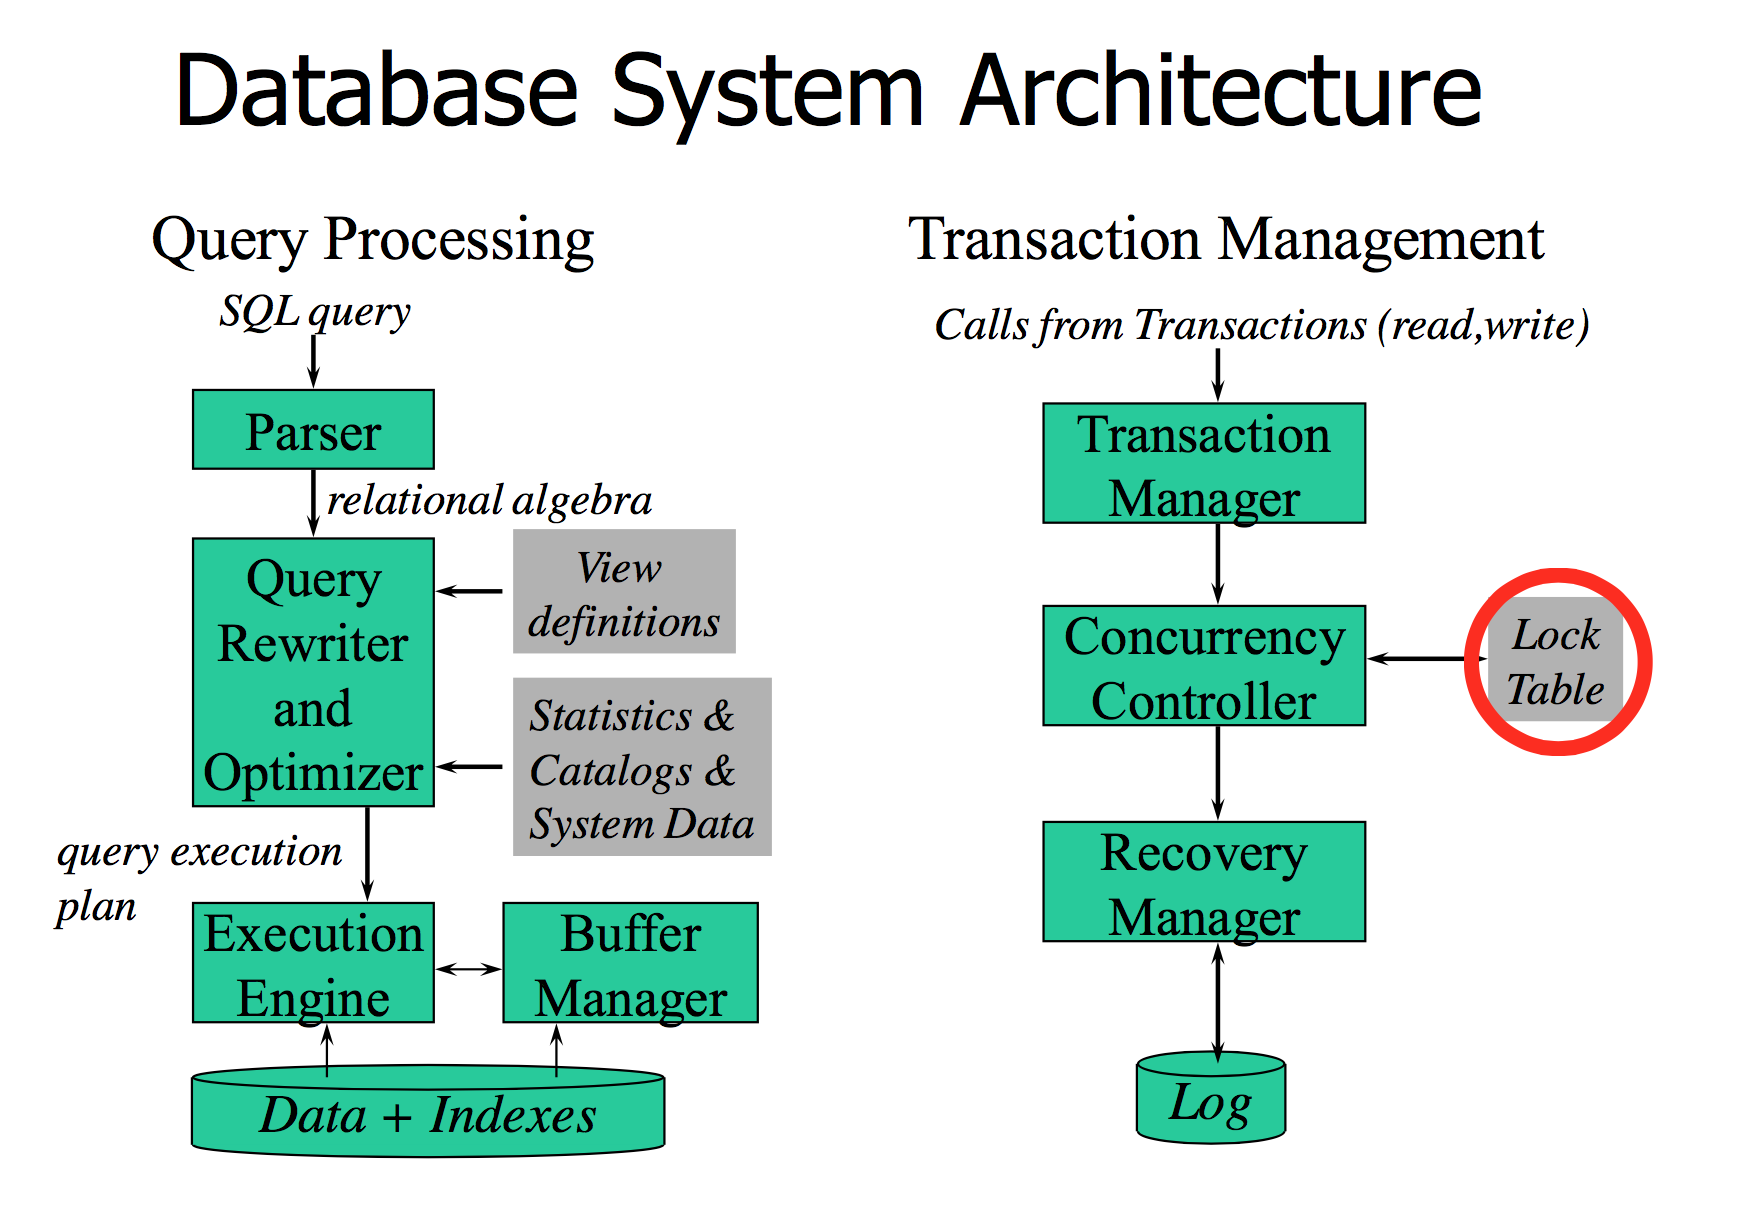
\includegraphics[height=2.5in]{img/db_sys_arch}}
\caption{CAPTION}
\label{fig:LABEL}
\end{figure}
\end{itemize}


\section{Hardware}
\begin{itemize}
\item Memory Hierarchy 
\begin{enumerate}
\item Blocked-based access 
\item Different Rates of Improvement 
\end{enumerate}
\item Tuned for blocks: Two-Phase, Multiway MergeSort (TPMMS). 
\begin{enumerate}
\item Phase 1: Load and sort into multiple lists 
\item Phase 2: Merge multiple lists 

Upper data size: 
$$
\frac{M^2}{B}
$$
, where $M\trieq$ RAM size, $B\trieq$ block size. 
\end{enumerate}
\end{itemize}


\section{Indexing}
\subsection{Conventional indexes}
\begin{enumerate}
\item Basic index types
  \begin{enumerate}
  \item Primary index
  \item Secondary index
  \end{enumerate}
  \begin{enumerate}
  \item Dense Index
  \item Spare Index
  \end{enumerate}
\item Multi-level indexes
\item Operations on conventional index
  \begin{enumerate}
  \item Duplication
  \item Deletion
  \item Insertion
  \end{enumerate}
\item Secondary Indexes
  \begin{enumerate}
  \item Non-sequencing \& multi-level
  \item Duplicate values
  
  Solutions:
    \begin{enumerate}
    \item Multiple index ptrs
    \item variable size of index list 
    \item chaining records 
    \item bucket (most used)
    \end{enumerate}
  \end{enumerate}
\end{enumerate}
\subsection{B+Tree}
\subsubsection{Bascis}
\begin{tabular}{lll}
\hline\noalign{\smallskip}
\textbf{Attrs} & \textbf{Non-leaf} & \textbf{Leaf} \\
\noalign{\smallskip}\hline\noalign{\smallskip}
Ptrs & \lceil\frac{n+1}{2}\rceil & \lfloor\frac{n+1}{2}\rfloor \\
\noalign{\smallskip}\hline\noalign{
\caption{Nodes at least half-full}
\end{tabular}
\subsubsection{Operations}
Core clues
\begin{enumerate}
\item \textbf{Split \& Up}: split half, move up the RIGHT node's FIRST of split nodes recursively
\item The node moved up should be removed in the original node UNLESS it is a leaf node. 
\end{enumerate}

\subsection{Hash}
\subsubsection{Extensible hashing}
Core clues:
\begin{enumerate}
\item Number of bit used $i$: $hash[:i]$.
\item When overflow:
  \begin{enumerate}
  \item \textbf{Expand} the index $i=i+1$.
  \item \textbf{Split} the bucket. Reorganized the split bucket according to new $i$.
  \item \textbf{Untouched} buckets remain untouched. 
  \end{enumerate}
\end{enumerate}
\begin{figure}[H]
        \centerline{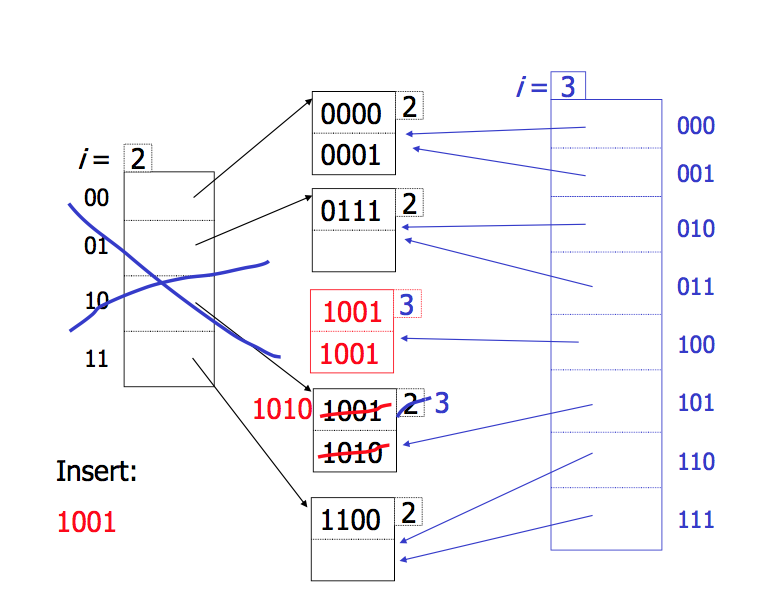
\includegraphics[height = 2in]{img/extensible_hashing}}
        \caption{Piazza}
    \label{fig:extensibleHashing}
\end{figure}
\subsection{BitMap}
Core clues:
\begin{enumerate}
\item gap count of 0's between 1's
\item encode length information [1]*(i-1)+[0], where i is number of bit for the gap count.
\item checksum: len info and gap count are of same size
\end{enumerate}


\section{Query Processing}
\subsection{Basic query processing}
\subsubsection{Relational algebra}\label{rlsAlgebra}
Notations:
\begin{enumerate}
\item $\sigma$: Filter, WHERE (conditions)
\item $\times$: Cartesian, FROM product 
\item $\Pi$: Projection, SELECT (attributes)
\item $x\ra y$: Extended projection, rename $x$ to $y$. Scalar func: $a+b\ra y$, String ops: $c||d \ra y$

\textbf{Scalar} functions: their input comes from the same tuple (as opp. \textbf{aggregate})
$$
\Pi_{x, y\ra z, x+y\ra w} R
$$
Alternatively, $PLUS_{x, y\ra z}$; similarly $CONCAT, MULT, CONCAT}$
\item $\bowtie$: Natural join: $R\bowtie S = \Pi_{distinctAttrs}\sigma_{condOnBoth}(R\times S)$. Notice that the $\times$ is \textbf{bag} version. 

$\bowtie_{\theta}$: $\triangleq \sigma_{\theta} (R\times S)$. $\theta$ is a condition. \item $\gamma$: Group and aggregation

\textbf{Aggregate} functions. 
$$
\gamma_{attr_{grpby}, aggrFn(attr) \ra attr'}
$$
Alternatively, $SUM_{attr_{grpby},aggrFn(attr)\ra attr'}$, similarly $AVG, MIN, MAX, COUNT$.
\item $\tau$: Order by. 

A result $o(exp)$ is ordered if
\begin{enumerate}
\item $o$ retains the originally ordered $exp$. (e.g. $\sigma$)
\item $o$ creates ordering. (e.g. ordered by pk, then iterative joining implt with FLY)
\end{enumerate}
$\sigma$ may retain the order generated by $\tau$ but depends on implementation. e.g. $\sigma^{FLY}$ may prodeces a ordered result. Discussion: 

$$
\tau_{R.A, R.B}\ \sigma_{R.B>5}^{FLY} R
$$
\begin{flushright}, produces a list\end{flushright}
$$
\sigma^{FLY}_{R.B>5}\ \tau_{R.A, R.B} R 
$$
\begin{flushright}, produces a bag but preserves the order.\end{flushright} 
\end{enumerate}
\subsubsection{Query Plan}
A simple SFW (Select From Where). 
\begin{enumerate}
\item Naive plan p:
$$
\Pi_{attr_1,attr_2}^{FLY}\Big[\sigma_{cond_R\wedge cond_S\wedge cond_{RS}}^{FLY} (R^{SCAN}\times S^{SCAN})\Big]
$$

FLY and SCAN are how exactly the plan is run.
\begin{enumerate}
\item \textbf{FLY}: on the fly, one entry at a time. Implementation: Iterator. No intermediate storage 
\item \textbf{SCAN}: scan the tables, one block at a time.
\begin{enumerate}
\item \textbf{Table-scan}. operator simply reads each block holding tuples of the relation.
\item \textbf{Index-scan}. uses an index to find tuples
\item \textbf{Sort-scan}. produces the tuples in sorted order.

\end{enumerate}}
\end{enumerate}

\item Join Plan (plan II):
$$
\Pi_{attrs} \Big[(\sigma_{cond_R}R)  \bowtie^{HASH} (\sigma_{cond_S}S) \Big]
$$
\item Index plan (plan III):

$$
\Pi_{attrs}\ \sigma_{cond_S}(\sigma_{cond_R}^{INDEX}R \bowtie^{RI} S)
$$
$\bowtie^{RI}$ Right Index Join. 
Steps:
\begin{enumerate}
\item Use index to get $\sigma$ based on condition on $R$. 
\item Right join $S$.
\item Filter based on condition on $S$.
\end{enumerate}
\end{enumerate}
\subsection{From query to optimal plan}
\begin{enumerate}
\item \textbf{lqp}. logical query plan $\equiv$ algebra ops 
\item Algebraic rewritings to transform the lqp
\item Physical Plan
\item Example:
\begin{itemize}
\item \textbf{``In'' Elimination}: 
\begin{lstlisting}
SELECT A.a
FROM A WHERE A.v IN (
    SELECT B.v
    FROM B
    WHERE cond_b
);
\end{lstlisting}
$In$ is transformed into $\sigma (A\times B)$. Then the basic algebra is:
$$
\Pi_{A.a}\ \sigma_{A.v=B.v}\quad (A \times \Pi \sigma B)
$$
Further optimized:
$$
\Pi_{A.a}(A \underset{A.v=B.v}\bowtie \Pi \sigma B)
$$

\end{itemize}
\end{enumerate}
\subsection{Bag algebra, list algebra, and extensions}
In this nodes, bag-version operations are assumed. 
\begin{enumerate}
\item Algebraic Operators (Bag Version) $\cup, \cap$
$$
R\cup S
$$
\item Convert to set (DISTINCT)
$$
\delta(R)
$$
\item Extended relational algebra - Section \ref{rlsAlgebra}.
\end{enumerate}
\subsection{Relational algebra optimization}
\begin{enumerate}
\item \rih{Commutativity and Associativity}
\begin{align*}
R \cdot S &= S\cdot R \\
R\cdot (S\cdot T) &= (R\cdot S) \cdot T \\
\end{align}

, where $o \in \{\times, \bowtie, \cup, \cap \}$  

proof: $R\times S = S\times R$
\begin{align*}
& R \times S \subset S \times R \\
& R \times S \supset S \times R \\
& \forall t, t\in R\times S,\mbox{ n times} \\
& r \in R\mbox{ m times}, s\in S \mbox{ k times}\\
& n = m*k \\
& \Ra\mbox{ find corresponding }t \in sr, k*m,\mbox{ n times} \\ 
& \therefore R \times S \subset S \times R \\
& \mbox{vice versa...}
\end{align*}
\rih{Logics}
\begin{align*}
\sigma_{cond_1\wedge cond_2}R &= \sigma_{cond_1}\ \sigma_{cond_2}R \\
\sigma_{cond_1\vee cond_2}R &= \sigma_{cond_1}R \cup \sigma_{cond_2}R
\end{align*}

\begin{flushright}, notice that $\vee$ only applies for set-version\end{flushright}

Decomposition of Negation:
TODO

\item \rih{Push $\sigma$} !important
$$
\sigma_{cond}(RoL) = (\sigma_{cond} R) o (\sigma_{cond} L) 
$$
\begin{flushright}, where $o\in \{-, \cup, \times, \bowtie\}$. \end{flushright}

\begin{itemize}
\item For $\{-\}$, it can directly drop the $\sigma_{cond}L$ to $L$. 
\item For $\{\times, \bowtie\}$, it can further drops the $\sigma_{cond}T$ to $T$ if the condition does not refer to attributes in $T$.
\end{itemize}

proof: $\sigma_{A=2}(R\bowtie S) = (\sigma_{A=2}R)\bowtie S$, given commutativity and $\sigma_{cond}(R\bowtie S) = R\bowtie \sigma_{cond}S$
\begin{align*}
\sigma_{A=2}(R\bowtie S) = \sigma_{A=2}(S\bowtie R) = S \bowtie (\sigma_{A=2}R)=(\sigma_{A=2}R\bowtie S)
\end{align*}

\rih{Combine $\pi$ \& $\sigma$}

This is a technique of proof by using axioms. 

\item \rih{Push $\pi$} 

\begin{align*}
& \pi_x (R \cup S) = \pi_x R \cup \pi_x S \\
& \pi_a (R \times S) = \pi_a (\pi_{cond1 \supset a}R \times \pi_{cond2 \supset a} S) \\
& \pi_a (R \bowtie S) = \pi_a(\pi_{cond1 \supset a \cup R.c}\ R \bowtie \pi_{cond2 \supset a\cup S.c}\ S) \\
& \pi_x R = \pi_x \pi_{y\supset x} R
\end{align*}
When denoting $\supset, \subset$, it is for AND composite. $cond1\supset a$ is a shorthand notation for $\{cond1|cond1 \supset a\}$

\item \rih{Aggregation} 

\begin{align*}
& \sigma_{cond\subset grpAttrs} \Sigma_{grpAttrs; attr\ra attr'} R = \Sigma_{grpAttrs, attr\ra attr'} \sigma_{cond\subset grpAttrs} R \\
& \Sigma_{GL;GA\ra RA} (R \cup S) = +_{RA1, RA2:RA} (\Sigma_{GL; GA\ra RA1 }R \bowtie \Sigma_{GL; GA\ra RA2} S)\\
& \Sigma_{GL2; RA1 \ra RA2} \Sigma_{GL1; GA \ra RA1} R = \Sigma_{GL2; GA\ra RA2} R
\end{align*}
Notation, in slides it is $grpList$ or $GL$ as $grpAttrs$; $SUM$ as $\Sigma$.
\item \rih{Cost, rule of thumb} 

\end{enumerate}
\subsection{Algorithms for Relational Algebra Operators}
\subsubsection{$\bowtie$}
\begin{enumerate}
\item Iteration join
\item Merge join 
\item Index join 
\item Hash join 
\end{enumerate}



%+Bibliography
\begin{thebibliography}{99}
\bibitem{Label1} ...
\bibitem{Label2} ...
\end{thebibliography}
%-Bibliography
\end{document}
